% !TeX program = lualatex
% !TeX encoding = utf8
% !TeX spellcheck = uk_UA
% !BIB program = biber

\documentclass[10pt]{beamer}
\usetheme{QuantumChemistry}
\usepackage{QuantumChemistry}
\addbibresource{../Bibliography/QuantumChemistry.bib}
\graphicspath{{pictures/}}

\title[Лекції з квантової хімії]{\huge\bfseries Природа хімічного зв'язку}
\subtitle{Лекції з квантової хімії}
\author{Пономаренко С. М.}
\date{}

\begin{document}
\pagestyle{empty}
%=======================================================================================================
\usebackgroundtemplate{
	\tikz\node[opacity=0.15]{\includegraphics[width=\paperwidth,height=\paperheight]{background}};%
}
\begin{frame}
	\titlepage
\end{frame}
%==========================================================================

\section{Теорія молекулярного іона водню. Метод МО ЛКАО}

\begin{frame}{Природа хімічного зв'язку}

	\only<1>{
		Існує два методи розрахунку структури та властивостей молекул:
		\begin{enumerate}
			\item Метод молекулярних орбіталей (МО-ЛКАО)
			\item Метод валентних зв'язків (ВЗ)
		\end{enumerate}
	}
	\only<2->{

		В методі МО-ЛКАО молекула розглядається з такої ж точки зору як і атом:
		\begin{enumerate}
			\item Кожному електрону в молекулі відповідає $\psi$-функція~--- молекулярна орбіталь
			\item Хвильова функція молекули характеризується набором квантових чисел
			\item Хвильовій функції відповідає енергія. Повна енергія молекули~--- енергія заповнених МО.
			\item Електронна структура молекули встановлюється принципами побудови (мінімуму енергії, Паулі, Гунда)
			\item Метод Хартрі-Фока для молекул
		\end{enumerate}
		\begin{center}
			\alert<3>{
				Ключ до розробки методу молекулярних орбіталей~--- задача про найпростішу молекулярну систему~--- молекулярний іон водню \ce{H^+_2}
			}
		\end{center}
	}




\end{frame}


\begin{frame}[t]{Молекулярний іон \ce{H^+_2}}{Гамільтоніан системи}
	\begin{columns}[c]
		\begin{column}{.4\linewidth}
			\vspace{0cm}
			\begin{overlayarea}{\textwidth}{0.7\textheight}
				\input{H2ion.tikz}
			\end{overlayarea}
		\end{column}
		\begin{column}{.6\linewidth}
			\begin{equation*}
				\hat H =  - \frac{\hbar^2}{2m} \nabla^2 - \frac{e^2}{r_a} - \frac{e^2}{r_b} + \frac{e^2}{R_{ab}}.
			\end{equation*}
			В атомній системі одиниць
			\begin{equation*}
				\hat H =  - \frac12 \nabla^2 - \frac{1}{r_a} - \frac{1}{r_b} + \frac{1}{R_{ab}}.
			\end{equation*}
			Рівняння Шредінґера
			\begin{equation*}\label{}
				\hat H \phi^\text{МО}(\vec{r}_a, \vec{r}_b | \vec{R}_{ab}) = E_e \phi^\text{МО}(\vec{r}_1, \vec{r}_2 | \vec{R}_{ab}),
			\end{equation*}
			де $\phi^\text{МО}(\vec{r}_1, \vec{r}_2 | \vec{R}_{ab})$~--- \alert{молекулярна орбіталь}.
		\end{column}
	\end{columns}
	\begin{alertblock}{}\scriptsize\centering
		Рівняння розв'язується точно (в еліптичній системі координат).

			[\fullcite{1508.01359}]
	\end{alertblock}
\end{frame}
%=======================================================================================================





%=======================================================================================================
\begin{frame}{Молекулярний іон \ce{H^+_2}}{Хвильові функції}
	\begin{columns}[c]
		\begin{column}{.3\linewidth}
			\begin{overlayarea}{\textwidth}{0.7\textheight}
				\input{H2ion.tikz}
			\end{overlayarea}
		\end{column}
		\begin{column}{.7\linewidth}

			\begin{block}{}\scriptsize
				Оскільки молекулярний іон \ce{H^+_2} --- єдина молекулярна система для якої можна отримати аналітичний розв'язок, то доцільно винайти наближення, яке б з високою точністю описало цю систему і вказало шлях для його використання для більш складних систем, для яких отримати точний аналітичний розв'язок вже неможливо.
			\end{block}

			\begin{block}{\small МО ЛКАО}
				Ідея наближення --- представити молекулярну орбіталь як лінійну комбінацію атомних орбіталей
			\end{block}
			\begin{equation*}
				\phi^\text{МО} = 1/\sqrt{2} (c_a \chi_{a}^\text{АО} +  c_b \chi_{b}^\text{АО})
			\end{equation*}
			Атомні орбіталі для \ce{H^+_2} можна взяти як для атома водню:
			\begin{equation*}\label{}
				\chi_a^\text{АО} = {1}/{\sqrt{\pi}}e^{-r_a}, \quad
				\chi_b^\text{АО} = {1}/{\sqrt{\pi}}e^{-r_b}.
			\end{equation*}
		\end{column}
	\end{columns}
\end{frame}
%=======================================================================================================





%=======================================================================================================
\begin{frame}[t]{Молекулярний іон \ce{H^+_2}}{Нормувальний множник та інтеграл перекриття}
	Реалізація МО ЛКАО:
	\begin{equation*}
		\phi_{S}^\text{МО} = \frac{c}{\sqrt{2}} \left( \chi_{a}^\text{АО} +  \chi_{b}^\text{АО}\right),\quad c_a =  c_b = c
	\end{equation*}
	\begin{equation*}
		\phi_{A}^\text{МО} = \frac{c}{\sqrt{2}}\left( \chi_{a}^\text{АО} -  \chi_{b}^\text{АО}\right), \quad c_a =  - c_b = c
	\end{equation*}
	\begin{multline*}
		\int\left| \phi_{S,A}^\text{МО}\right|^2 dV
		= \frac{c^2}{2}\left( \int\left| \chi_{a}^\text{АО}\right|^2 dV + \int\left| \chi_{b}^\text{АО}\right|^2 dV  \pm
		2 \int\chi_{a}^\text{АО} \chi_{b}^\text{АО} dV \right) = \\
		= \frac{c^2}{2} \left( 2 \pm 2\int\chi_a^\text{АО}\phi_b^\text{АО} dV \right) = c^2 \left( 1 \pm  S \right) = 1
	\end{multline*}
	\begin{overprint}
		\onslide<1>
		де $S$ -- інтеграл перекриття (перекриття орбіталей \alert{одного і того ж електрона}):
		\begin{equation*}
			S = \int\chi_a^\text{АО}\chi_b^\text{АО}dV
		\end{equation*}
		\onslide<2>
		Нормувальний множник:
		\begin{equation*}
			c = \frac{1}{\sqrt{(1\pm S)}}
		\end{equation*}
	\end{overprint}

\end{frame}
%=======================================================================================================
\begin{frame}{Молекулярний іон \ce{H^+_2}}{Інтеграл перекриття. Фізичний смисл}
	\begin{alertblock}{}\itshape\centering
		Для утворення хімічного зв'язку -- необхідне перекривання хвильових функцій (атомних орбіталей)!
	\end{alertblock}

	Перекриття атомних орбіталей залежить від відстані між атомами:\\
	при $R_{ab} \to \infty$, $S \to 0$,
	при $R_{ab} \to 0$, $S \to 1$.
	\begin{equation*}
		\tcbhighmath[drop fuzzy shadow]{S = e^{-R_{ab}}\left( 1 + R_{ab} +\frac13 R_{ab}^2\right)}
	\end{equation*}
	\begin{overprint}
		\onslide<1>
		\begin{center}
			\begin{tikzpicture}[scale=0.7]
				\begin{axis}[axis lines = middle, clip=false,
						ylabel={$S$},
						y label style={at={(axis description cs:-0.01,1)},anchor=east},
						xlabel={$R_{ab}$},
						x label style={at={(axis description cs:1,0)},anchor=west},
						xmin=0, xmax=10,
						ymin=0, ymax=1.20,
						width = 10cm,
						height = 5cm,
						ticks=none,
					]
					\addplot[thick,	domain=0:9,
						%restrict y to domain={0:1},
						red,
						thick,
						samples=500, legend entry=$S$] {exp(-x)*(1+x + x^2/3)};
				\end{axis}
			\end{tikzpicture}
		\end{center}
		\onslide<2>
		\noindent%
		\begin{tikzpicture}[scale=0.9]
			\coordinate (x0) at (0,0);
			\coordinate (x1) at (0.5,0);

			\shade[even odd rule, inner color=red,outer color=red!20 ,fill opacity=0.3] (x0) circle (1);
			\shade[even odd rule, inner color=red,outer color=red!20, fill opacity=0.3] (x1) circle (1);
			\node at (x0) {\textbullet};
			\node[below left=25pt of x0] {$\phi_a$};
			\node at (x1) {\textbullet};
			\node[below right=25pt of x1] {$\phi_b$};
			\node[below] at (0.25, -1.1) {$S_{ab} \approx 1$};
			\draw[latex-latex, gray] (x0) -- node[below] {$R_{ab}$}(x1);
			%==========================================================
			\coordinate (y0) at (3.5,0);
			\coordinate (y1) at (5,0);

			\shade[even odd rule, inner color=red,outer color=red!20 ,fill opacity=0.3] (y0) circle (1);
			\shade[even odd rule, inner color=red,outer color=red!20 ,fill opacity=0.3] (y1) circle (1);
			\node at (y0) {\textbullet};
			\node[below left=25pt of y0] {$\phi_a$};
			\node at (y1) {\textbullet};
			\node[below right=25pt of y1] {$\phi_b$};
			\node[below] at (4.25, -1.1) {$0 < S_{ab} < 1$};
			\draw[latex-latex, gray] (y0) -- node[below] {$R_{ab}$}(y1);
			%==========================================================
			\coordinate (z0) at (7.5,0);
			\coordinate (z1) at (9.75,0);

			\shade[even odd rule, inner color=red,outer color=red!20 ,fill opacity=0.3] (z0) circle (1);
			\shade[even odd rule, inner color=red,outer color=red!20 ,fill opacity=0.3] (z1) circle (1);
			\node at (z0) {\textbullet};
			\node[below left=25pt of z0] {$\phi_a$};
			\node at (z1) {\textbullet};
			\node[below right=25pt of z1] {$\phi_b$};
			\node[below] at (8.625, -1.1) {$S_{ab} \approx 0$};
			\draw[latex-latex, gray] (z0) -- node[below] {$R_{ab}$}(z1);
		\end{tikzpicture}
	\end{overprint}

\end{frame}
%=======================================================================================================
\begin{frame}{Молекулярний іон \ce{H^+_2}}{Молекулярні орбіталі}
	\begin{columns}[c]
		\begin{column}{.4\linewidth}
			\begin{overlayarea}{\textwidth}{0.7\textheight}
				\input{H2ion.tikz}
			\end{overlayarea}
		\end{column}
		\begin{column}{.6\linewidth}
			\begin{overprint}
				\onslide<1>
				Симетрична та антисиметрична $\phi$-функції, утворені за допомогою одноелектронних $\chi$-функцій~---~\alert{атомних орбіталей} ---~називаються \alert{молекулярними орбіталями}:
				\begin{align*}
					\phi_{S}^\text{МО} = \frac{1}{\sqrt{2(1+S)}}\left( \chi_{a}^\text{АО} +  \chi_{b}^\text{АО}\right) \\
					\phi_{A}^\text{МО} = \frac{1}{\sqrt{2(1-S)}}\left( \chi_{a}^\text{АО} - \chi_{b}^\text{АО}\right)  \\
				\end{align*}
				\onslide<2>

				\begin{block}{}
					Метод молекулярних орбіталей (метод МО)~--- це метод наближеного розв'язання електронного рівняння Шредингера для багатоелектронних молекулярних систем.

					\medskip

					Ґрунтується на побудові повної хвильової функції у вигляді антисиметризованого добутку молекулярних орбіталей (детермінант Слейтера).

					\medskip

					Молекулярні орбіталі, у свою чергу, зазвичай представляють як лінійні комбінації атомних орбіталей (наближення \alert{МО ЛКАО}).

				\end{block}
			\end{overprint}
		\end{column}
	\end{columns}
\end{frame}


%=======================================================================================================
\begin{frame}{Молекулярний іон \ce{H^+_2}}{Енергія системи}
	При розрахунку енергії за формулою:
	\begin{equation*}
		E_{S,A} = \opbracket{\phi_{S,A}}{\hat H}{\phi_{S,A}} = \frac{H_{aa} \pm H_{bb}}{1\pm S},
	\end{equation*}
	\begin{overprint}
		\onslide<1>
		Розглянемо інтеграли:
		\begin{align*}
			H_{aa} = H_{bb}  & = \opbracket{\phi_{a}}{\hat H}{\chi_{a}} = \opbracket{\chi_{b}}{\hat H}{\chi_{b}} \\
			H_{ab}  = H_{ba} & = \opbracket{\chi_{a}}{\hat H}{\chi_{b}}
		\end{align*}
		\onslide<2>
		\begin{equation*}
			H_{aa} = \opbracket{\chi_{a}}{\hat H}{\chi_{a}} = \opbracket{\chi_{a}}{\hat H_a - \frac{1}{r_b} + \frac{e^2}{R_{ab}}}{\chi_{a}} 		= E_H + J + \frac{1}{R_{ab}},
		\end{equation*}
		де \(J = \opbracket{\chi_{a}}{-\frac{e^2}{r_b}}{\chi_{a}}\) --- кулонівський інтеграл.
		\onslide<3>
		\begin{equation*}
			H_{ab} = \opbracket{\chi_{a}}{\hat H}{\chi_{b}} = \opbracket{\chi_{a}}{\hat H_a - \frac{e^2}{r_b} + \frac{e^2}{R_{ab}}}{\chi_{b}} =  E_HS + \beta + \frac{1}{R_{ab}}S,
		\end{equation*}
		де \(\beta = \opbracket{\chi_{a}}{-\frac{e^2}{r_b}}{\chi_{b}}\) --- резонансний інтеграл.
		\onslide<4>
		Повна енергія системи дорівнює:
		\begin{equation*}
			E(R_{ab}) = E_H + \frac{e^2}{R_{ab}} + \frac{J\pm\beta}{1\pm S}
		\end{equation*}
	\end{overprint}
\end{frame}

%=======================================================================================================
\begin{frame}{Молекулярний іон \ce{H^+_2}}{Значення інтегралів}
	\[
		\beta = -e^{-R_{ab}}(1 + R_{ab}) \qquad J  = - \frac{1}{R_{ab}}\left[ 1 - e^{-2R_{ab}}(1 + R_{ab})\right]
	\]
	\begin{center}
		\begin{tikzpicture}[]
			\begin{axis}[axis lines = middle, clip=false,
					ylabel={$J$, $\beta$},
					y label style={at={(axis description cs:-0.01,1)},anchor=east},
					xlabel={$R_{ab}$},
					x label style={at={(axis description cs:1,0.5)},anchor=west},
					xmin=0, xmax=2,
					ymin=-1.20, ymax=1.20,
					width = 10cm,
					height = 6cm,
					ticks=none,
				]
				\addplot[thick,	domain=0:2,
					%restrict y to domain={0:1},
					red,
					thick,
					samples=500, legend entry=$\beta$] {-exp(-x)*(1+x)};
				\addplot[thick,	domain=0.01:2,
					%restrict y to domain={0:1},
					blue,
					thick,
					samples=500,legend entry=$J$] {-1/x*(1-exp(-2*x)*(1+x))};
			\end{axis}
		\end{tikzpicture}

		При $R_{ab} \to 0$, $\beta = -1$, $J = -1$
	\end{center}
\end{frame}

%============================================================================
\begin{frame}{Молекулярний іон \ce{H^+_2}}{Енергія системи в залежності від міжядерної відстані}
	\begin{center}
		\begin{tikzpicture}[scale=1.75]
			\draw[-latex] (-0.3,0) -- ++(3.8,0) node[below] {$R_{ab}$};
			\draw[-latex] (0,-2.5) -- ++(0,4) node[left] {$E$};
			\draw[domain=0.3:3.2, smooth, variable=\x, red, samples = 100]  plot ({\x}, {-3/\x + 1/(\x*\x)});
			\draw[domain=0.8:3.2, smooth, variable=\x, blue, samples = 100]  plot ({\x}, {1/(\x*\x)});
			\def\i{1.4}
			\node[circle, fill=red, inner sep= 2pt] (A) at ({\i}, {-3/\i + 1/(\i*\i)}) {};
			\node[circle, fill=blue, inner sep= 2pt] (B) at ({\i}, {1/(\i*\i)}) {};
			\draw[dashed] (B) -- +(20:1) node[anchor=south west] {$E_{A} = E_H + \frac{1}{R_{ab}} + \frac{J-\beta}{1- S}$} ;
			\draw[dashed] (A) -- +(-20:1) node[anchor=south west] {$E_{S} = E_H + \frac{1}{R_{ab}} + \frac{J+\beta}{1+ S}$} ;
			%    \draw[dashed] (A) |- node[above] {$R_{\ci}$} (0,0) ;
		\end{tikzpicture}%
	\end{center}
	%---------------------------------------------------------
\end{frame}
%============================================================================

%=======================================================================================================
\begin{frame}{Молекулярний іон \ce{H^+_2}}{Зв'язуюча та розрихлююча орбіталі}
	\begin{columns}[c]
		\begin{column}{.5\linewidth}
			\includegraphics[width=0.9\linewidth]{H2Bond_antibond}
		\end{column}
		\begin{column}{.5\linewidth}
			\begin{overprint}
				\onslide<1>
				Зниження енергії системи \\(утворення зв'язку):
				\begin{equation*}
					\phi_{S} = \frac{1}{\sqrt{2(1+S)}}\left( \chi_{a} +  \chi_{b}\right)
				\end{equation*}
				\begin{equation*}
					\Delta E = E - E_H = \frac{e^2}{R_{ab}} + \frac{J+\beta}{1 + S}
				\end{equation*}
				Підвищення енергії системи \\(зв'язок не утворюється):
				\begin{equation*}
					\phi_{A} = \frac{1}{\sqrt{2(1-S)}}\left( \chi_{a} -  \chi_{b}\right)
				\end{equation*}
				\begin{equation*}
					\Delta E = E - E_H = \frac{e^2}{R_{ab}} + \frac{J-\beta}{1- S}
				\end{equation*}
				\onslide<2>
				\begin{equation*}
					\phi_{A} = \frac{1}{\sqrt{2(1-S)}}\left( \chi_{a} -  \chi_{b}\right)
				\end{equation*}
				Зв'язок в стані, що описувється функцією $\Psi_A$, не утворюється.
				Така молекулярна орбіталь  називається
				антизв'язуючою, або \alert{розрихлюючою}.
				\begin{equation*}
					\phi_{S} = \frac{1}{\sqrt{2(1+S)}}\left( \chi_{a} +  \chi_{b}\right)
				\end{equation*}
				Відповідно орбиталь що описувється функцією $\Phi_S$ називається  \alert{зв'язуючою}.
			\end{overprint}
		\end{column}
	\end{columns}
\end{frame}

\begin{frame}{Молекулярний іон \ce{H^+_2}}{Кватново-механічна інтерференція}
	\begin{figure}[h!]
		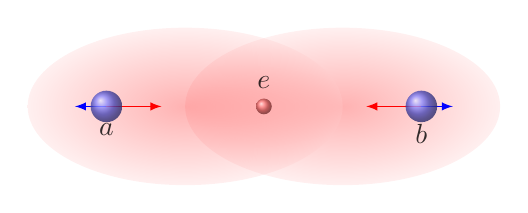
\begin{tikzpicture}
			%coordinates
			\coordinate (N1) at (-2,0);
			\coordinate (N2) at (2,0);
			\coordinate (e) at (0,0);
			%Vectors
			\begin{scope}
				\shade[even odd rule, inner color=red,outer color=red!20 ,fill opacity=0.3] ([xshift=-1cm]N2) ellipse (2 and 1);
				\shade[even odd rule, inner color=red,outer color=red!20 ,fill opacity=0.3] ([xshift=1cm]N1) ellipse (2 and 1);
				\draw[-latex, red] (N1) -- ([xshift=0.7cm]N1);
				\draw[-latex, red] (N2) -- ([xshift=-0.7cm]N2);

				\draw[-latex, blue] (N1) -- ([xshift=-0.4cm]N1);
				\draw[-latex, blue] (N2) -- ([xshift=+0.4cm]N2);
			\end{scope}
			%Nuclei
			\shade[ball color=blue!60!white,opacity=0.80] (N1) node[below=0.1cm]  {$a$} circle (0.2cm);
			\shade[ball color=blue!60!white,opacity=0.80] (N2) node[below=0.1cm]  {$b$} circle (0.2cm);
			%Electrons
			\shade[ball color=red!60!white,opacity=0.80]  (e) node[above=0.1cm]  {$e$} circle (0.1cm);
		\end{tikzpicture}
		\caption{Електрон перебуває між ядрами. Утворюється зв'язок}
	\end{figure}
	\begin{figure}[h!]
		\begin{tikzpicture}
			%coordinates
			\coordinate (N1) at (-2,0);
			\coordinate (N2) at (2,0);
			\coordinate (e) at (-3,0);
			\coordinate (ve) at (3,0);
			%Vectors
			\begin{scope}
				\shade[even odd rule, inner color=red,outer color=red!20 ,fill opacity=0.3] ([xshift=1cm]N2) ellipse (2 and 1);
				\shade[even odd rule, inner color=red,outer color=red!20 ,fill opacity=0.3] ([xshift=-1cm]N1) ellipse (2 and 1);
				\draw[-latex, red] (N1) -- ([xshift=-0.7cm]N1);
				\draw[-latex, red] (N2) -- ([xshift=0.7cm]N2);

				\draw[-latex, blue] (N1) -- ([xshift=-0.4cm]N1);
				\draw[-latex, blue] (N2) -- ([xshift=+0.4cm]N2);
				\draw[latex-latex, dashed, gray] (e) to[bend left] node[above] {\tiny одночасно}(ve);
			\end{scope}
			%Nuclei
			\shade[ball color=blue!60!white,opacity=0.80] (N1) node[below=0.1cm]  {$a$} circle (0.2cm);
			\shade[ball color=blue!60!white,opacity=0.80] (N2) node[below=0.1cm]  {$b$} circle (0.2cm);
			%Electrons
			\shade[ball color=red!60!white,opacity=0.80]  (e) node[above=0.1cm]  {$e$} circle (0.1cm);
			\shade[ball color=red!60!white,opacity=0.80, dashed]  (ve) node[above=0.1cm]  {$e$} circle (0.1cm);
		\end{tikzpicture}
		\caption{Електрон перебуває поза ядрами. Зв'язку немає}
	\end{figure}
\end{frame}

%=======================================================================================================
%\begin{frame}
%	\frametitle{Молекула \ce{H2}}
%	\framesubtitle{Енергія молекули водню з урахуванням тотожності електронів}
%	\begin{columns}[c]
%		\begin{column}{.6\linewidth}
%			\includegraphics[width=1\linewidth]{H2Econj}
%		\end{column}
%		\begin{column}{.4\linewidth}
%			\includegraphics[width=1\linewidth]{H2Bond_antibond}
%		\end{column}
%	\end{columns}
%\end{frame}

\begin{frame}{Типи молекулярних орбіталей}
	У двоатомной молекулі вже існує обраний напрям (вісь симетрії)~--- лінія зв'язку між молекулами (вісь $z$).

	\begin{center}
		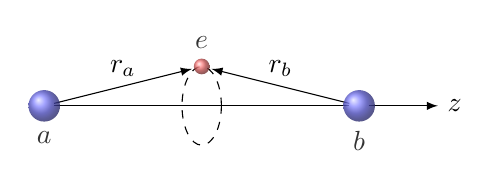
\begin{tikzpicture}
			%coordinates
			\node (N1) at (-2,0) {};
			\node (N2) at (2,0) {};
			\node (e) at (0,0.5) {};
			%Vectors
			\begin{scope}
				\draw[-latex] (N1) -- (N2) -- (3,0) node[right] {$z$};
				\draw[-latex] (N1) -- node[above] {$r_{a}$} (e);
				\draw[-latex] (N2) -- node[above] {$r_{b}$} (e);
				\draw[dashed] (0,0) ellipse(0.25 and 0.5);
			\end{scope}
			%Nuclei
			\shade[ball color=blue!60!white,opacity=0.80] (N1) node[below=0.2cm]  {$a$} circle (0.2cm);
			\shade[ball color=blue!60!white,opacity=0.80] (N2) node[below=0.2cm]  {$b$} circle (0.2cm);
			%Electrons
			\shade[ball color=red!60!white,opacity=0.80]  (e) node[above=0.1cm]  {$e$} circle (0.1cm);
		\end{tikzpicture}
	\end{center}

	Квантове число \[\lambda = \left| m\right| \] визначає проекцію орбітального моменту 	імпульсу електрона на вісь $z$~--- лінію, що сполучає ядра молекули.

	Стани з значеннями $\lambda$ позначають літерами грецького алфавіту:

	\begin{table}[htbp!]
		\begin{tblr}{
				colspec={Q[l,m]|cccc},
				cell{1}{1-6} = {cyan!50},
			}
			\hline
			Значення $\lambda$ & 0        & 1     & 2        & 3      & 4        \\ \hline
			Позначення         & $\sigma$ & $\pi$ & $\delta$ & $\phi$ & $\gamma$ \\ \hline
		\end{tblr}
	\end{table}
\end{frame}

\begin{frame}{Молекулярні орбіталі \ce{H^+_2}}{Симетрія}
	\begin{figure}
		\centering
		\includegraphics[width=0.7\linewidth]{sigma_MO}
		\caption{Ізоповерхні величини $|\phi|$ для $\sigma_g$ (ліворуч) та $\sigma^*_u$ (праворуч) молекулярних орбіталей молекулярного іона \ce{H^+_2}.}
		\label{fig:sigmamo}
	\end{figure}
	\begin{overprint}
		\onslide<1>
		$\sigma_g$ --- зв'язуюча $\sigma$-молекeкулярна орбіталь (індекс $g$ --- означає gerade (нім. парний))

		$\sigma^*_u$ --- розрихлююча $\sigma$-молекeкулярна орбіталь (індекс $u$ --- означає ungerade (нім. непарний))
		\onslide<2>
		Канонічні молекулярні орбіталі делокалізовані по всій молекулі. Це діаметрально протилежно до локалізованого двохелектронного зв'язку, яким оперує \alert{метод валентних зв'язків. }
	\end{overprint}
\end{frame}

\begin{frame}{Перекривання молекулярних орбіталей}
	\begin{columns}[c]
		\begin{column}{.6\linewidth}
			\begin{figure}
				\centering
				\begin{tikzpicture}[scale=0.4]
					\pgfgettransformentries{\a}{\b}{\c}{\d}{\xtrans}{\ytrans}
					\node[anchor=south west,inner sep=0] (image) at (0,0) {\includegraphics[scale=\a]{formas-orbitales}};
					\begin{scope}[x={(image.south east)},y={(image.north west)}]
						%		\draw[help lines,xstep=.1,ystep=.1] (0,0) grid (1,1);
						%		\foreach \x in {0,1,...,10} { \node [anchor=north] at (\x/10,0) {\x}; }
						%		\foreach \y in {0,1,...,10} { \node [anchor=east] at (0,\y/10) {\y}; }
						\node at (0.85,0.88) {$\sigma_gs$};
						\node at (0.85,0.75) {$\sigma_u^*s$};
						\node at (0.85,0.62) {$\sigma_gp$};
						\node at (0.85,0.48) {$\sigma_u^*p$};
						\node at (0.85,0.30) {$\pi_up$};
						\node at (0.85,0.12) {$\pi_g^*p$};
					\end{scope}
				\end{tikzpicture}
				\caption{Вигляд $\sigma$- та $\pi$-молекулярних орбіталей}
				\label{fig:formas-orbitales}
			\end{figure}
		\end{column}
		\begin{column}{.4\linewidth}
			$s$-атомні орбіталі можуть утворити лише $\sigma$-молекулярні орбіталі.

			\vspace*{1em}

			$p$-атомні орбіталі можуть утворити $\sigma$- та $\pi$-молекулярні орбіталі.

			\vspace*{1em}

			$d$-атомні орбіталі можуть утворити $\sigma$-, $\pi$- та $\delta$-молекулярні орбіталі.

			\vspace*{1em}

			$\ldots$
		\end{column}
	\end{columns}


\end{frame}
\begin{frame}{Принцип побудови молекулярних орбіталей}
	\begin{enumerate}
		\item Одноелектронне наближення в атомах дозволило використовувати принцип побудови для атомів і пояснити структуру.

		\item Воднеподібні орбіталі у багатоелектронних атомах довелося дещо змінити
		      з урахуванням впливу міжелектронного відштовхування (зняття
		      виродження по $l$ тощо).

		\item Точно так одноелектронне наближення в молекулах~--- молекулярні орбіталі, отримані при розв'язку задачі для \ce{H^+_2} можна взяти за основу і використовувати в багатоелектронних системах з відповідними <<виправленнями>>.

		\item Основою для <<виправлення>> служать вже АО, для реальних атомів $2s$-рівень, наприклад, розташований нижче $2р$ тощо.

		\item Принцип побудови для молекул ґрунтується на тих же засадах,
		      що і для атомів~--- енергетичний критерій, принцип Паулі, правило Гунда.

\begin{block}{}\scriptsize
    		  Електрони прагнуть зайняти найбільш низько розташовані МО,
		      але принцип Паулі не дозволяє розташовуватися на одній МО більш, ніж
		      двом електронам (з протилежними спинами).
\end{block}
	\end{enumerate}
\end{frame}

\begin{frame}{Схема МО \ce{H^+_2}}
	\framesubtitle<1>{Електронна конфігурація молекул}
	\only<1>{
		Подібно до того, як ми представляли електронну конфігурацію атомів шляхом заповнення орбіталей (наприклад, $1s^22s^2$), так ми будемо представляти двоатомні молекули шляхом заповнення орбіталей, що призводить до молекулярних електронних конфігурацій, таких, наприклад як
		\[
			(\sigma_g1s)^2(\sigma^*_u1s)^2
		\]
	}
	\only<2->{
		\begin{center}
			\begin{MOdiagram}[style = fancy, distance = 7cm, AO-width = 15pt,names, labels]
				\atom[H]{left}{1s=0}
				\atom[H]{right}{1s=0}
				\only<2>{\molecule[\ce{H2}]{1sMO={1.5;up}}}
				\only<3>{\molecule[\ce{H2}]{1sMO={1.5;,up}, color = {1sigma*=red}}}
				\EnergyAxis[title=E,head=stealth]
			\end{MOdiagram}
			\vspace*{2em}

			\only<2>{$(\sigma_g1s)^1$}
			\only<3>{$(\sigma^*_u1s)^1$}
		\end{center}
	}
\end{frame}


\begin{frame}{Схема МО для гомоядерних двоатомних молекул}
	\framesubtitle<1>{Молекула \ce{H2}}
	\framesubtitle<2>{Молекула \ce{He2}}
	\begin{overprint}
		\onslide<1>
		\begin{center}
			\begin{MOdiagram}[style = fancy, distance = 7cm, AO-width = 15pt,names, labels]
				\atom[H]{left}{1s={;up}}
				\atom[H]{right}{1s={;down}}
				\molecule[\ce{H-H}]{1sMO={1.5;pair}}
				\EnergyAxis[title=E,head=stealth]
			\end{MOdiagram}
			\[
				(\sigma_g1s)^2
			\]
		\end{center}
		\onslide<2>
		\begin{center}
			\begin{MOdiagram}[style = fancy, distance = 7cm, AO-width = 15pt,names, labels]
				\atom[He]{left}{1s={;pair}}
				\atom[He]{right}{1s={;pair}}
				\molecule[\ce{He2}]{1sMO={1.5;pair, pair},
					color = { 1sigma*=red }}
				\EnergyAxis[title=E,head=stealth]
			\end{MOdiagram}
			\[
				(\sigma_g1s)^2(\sigma^*_u1s)^2
			\]
		\end{center}
		\begin{center}
			Молекула за нормальних умов не виникає.
		\end{center}
	\end{overprint}
\end{frame}

\begin{frame}{Кореляційна діаграма для двоатомних молекул}
	\emph{Кореляційні діаграми} показують, як змінюється енергія орбіталі при зміні міжатомної відстані.
	\begin{columns}[T]
		\begin{column}{.45\linewidth}
			\begin{overlayarea}{\textwidth}{0.7\textheight}
				\includegraphics[width=1\linewidth]{Correlation_Diagram}
			\end{overlayarea}
		\end{column}
		\begin{column}{.5\linewidth}
			\vspace*{2em}

			\begin{block}{}
                Розрихлюючі орбіталі завжди відповідають орбіталям об'єднаного атома з більшим головним квантовим числом (промотув\'{а}ння).
            \end{block}

			\begin{block}{Правило неперетинання}\small
				Енергії МО з однаковою симетрією не можуть перетинатися.
			\end{block}

		\end{column}
	\end{columns}

\end{frame}

\begin{frame}{Схема МО для гомоядерних двоатомних молекул другого періоду}
	\begin{overprint}
		\onslide<1>
		%============================== Li ======================
		\begin{center}
			\scalebox{0.8}{
				\begin{MOdiagram}[style=square, labels,names,AO-width=8pt,labels-fs=\footnotesize]
					\atom[\ce{Li_a}]{left}{
						1s  = {;pair},
						2s  = {;up},
						%2p = {;}
					}
					\atom[\ce{Li\bond{1}Li}]{right}{
						1s  = {;pair},
						2s  = {;down},
						%2p = {;}
					}
					\molecule[\ce{Li2}]{
						1sMO = {;pair,pair},
						2sMO = {;pair},
						%2pMO = {;},
						color = { 1sigma*=red, 2sigma*=red }
					}
					\EnergyAxis
				\end{MOdiagram}
			}

			Електронна конфігурація молекули \ce{Li2}
			\[
				(\sigma_g1s)^2(\sigma^*_u1s)^2(\sigma_g2s)^2
			\]

		\end{center}
		%============================== Be ======================
		\onslide<2>
		\begin{center}
			\scalebox{0.8}{
				\begin{MOdiagram}[style=square, labels,names,AO-width=8pt,labels-fs=\footnotesize]
					\atom[a]{left}{
						1s  = {;pair},
						2s  = {;pair},
						%2p = {;}
					}
					\atom[b]{right}{
						1s  = {;pair},
						2s  = {;pair},
						%2p = {;}
					}
					\molecule[\ce{Be2}]{
						1sMO = {;pair,pair},
						2sMO = {;pair,pair},
						%2pMO = {;},
						color = { 1sigma*=red, 2sigma*=red }
					}
					\EnergyAxis
				\end{MOdiagram}
			}

			Електронна конфігурація молекули \ce{Be2}
			\[
				(\sigma_g1s)^2(\sigma^*_u1s)^2(\sigma_g2s)^2(\sigma^*_u2s)^2
			\]
			Молекула нестабільна і за нормальних умов не виникає.
		\end{center}
	\end{overprint}
	\framesubtitle<1>{Молекула \ce{Li2}}
	\framesubtitle<2>{Молекула \ce{Be2}}
\end{frame}

\begin{frame}{Схема МО для гомоядерних двоатомних молекул}
	\MOsetup{
		style=square,
		labels,
		names,
		AO-width=8pt,
		labels-fs=\footnotesize,
		labels-style={blue}
	}
	\begin{overprint}
		%============================== B2 ======================
		\onslide<1>
		\begin{columns}[T]
			\begin{column}{.45\linewidth}
				\scalebox{0.7}{
					\begin{MOdiagram}
						\atom[\ce{a}]{left}{
							1s  = {;pair},
							2s  = {;pair},
							2p = {;up}
						}
						\atom[\ce{b}]{right}{
							1s  = {;pair},
							2s  = {;pair},
							2p = {;up}
						}
						\molecule[\ce{B\bond{1}B}]{
							1sMO = {;pair,pair},
							2sMO = {;pair,pair},
							2pMO = {0.5/1.5,1.5/0.5;,up,up},
							color = { 1sigma*=red, 2sigma*=red }
						}
						\EnergyAxis
					\end{MOdiagram}
					%	    \begin{tikzpicture}[overlay]
					%	          \node[arrow box, draw, red, arrow box arrows={east:1.9cm},
					%	          text width=2.4em, minimum height=3.4ex]
					%	          at (1,4) {Парамагнетизм};
					%	    \end{tikzpicture}
				}
			\end{column}
			\begin{column}{.5\linewidth}

				Електронна конфігурація молекули \ce{B2}
				\[
					(\sigma_g1s)^2(\sigma^*_u1s)^2(\sigma_g2s)^2(\sigma^*_u2s)^2(\pi_u2p)^2
				\]

				Із-за двох неспарених електронів, які знаходяться на $2\pi_y$ та $2\pi_z$ орбіталях, молекула \ce{B2} є \alert{парамагнітною}.

				\vspace*{2em}

				{\footnotesize Чому на орбіталях $2\pi_y$ та $2\pi_z$ розташовані електрони з однаковим напрямком спіну? Що їм забороняє сісти на різні орбіталі з різними напрямками спіну?}


			\end{column}
		\end{columns}
		%============================== C2 ======================
		\onslide<2>
		\begin{columns}[T]
			\begin{column}{.45\linewidth}
				\scalebox{0.7}{
					\begin{MOdiagram}
						\atom[\ce{a}]{left}{
							1s  = {;pair},
							2s  = {;pair},
							2p = {;up,up}
						}
						\atom[\ce{b}]{right}{
							1s  = {;pair},
							2s  = {;pair},
							2p = {;up,up}
						}
						\molecule[\ce{C\bond{2}C}]{
							1sMO = {;pair,pair},
							2sMO = {;pair,pair},
							2pMO = {0.5/1.5,1.5/0.5;,pair,pair},
							color = { 1sigma*=red, 2sigma*=red }
						}
						\EnergyAxis
					\end{MOdiagram}
				}
			\end{column}
			\begin{column}{.5\linewidth}

				Електронна конфігурація молекули \ce{C2}
				\[
					(\sigma_g1s)^2(\sigma^*_u1s)^2(\sigma_g2s)^2(\sigma^*_u2s)^2(\pi_u2p)^4
				\]

				%				Основний терм: ${}^1\Sigma^+_g$

			\end{column}
		\end{columns}
		%============================== N2 ======================
		\onslide<3>
		\begin{columns}[T]
			\begin{column}{.45\linewidth}
				\scalebox{0.7}{
					\begin{MOdiagram}
						\atom[\ce{a}]{left}{
							1s  = {;pair},
							2s  = {;pair},
							2p = {;up,up,up}
						}
						\atom[\ce{b}]{right}{
							1s  = {;pair},
							2s  = {;pair},
							2p = {;up,up,up}
						}
						\molecule[\ce{N\bond{3}N}]{
							1sMO = {;pair,pair},
							2sMO = {;pair,pair},
							2pMO = {0.5/1.5,1.5/0.5;pair,pair,pair},
							color = { 1sigma*=red, 2sigma*=red }
						}
						\EnergyAxis
					\end{MOdiagram}
				}
			\end{column}
			\begin{column}{.5\linewidth}

				Електронна конфігурація молекули \ce{N2}
				\begin{multline*}
					(\sigma_g1s)^2(\sigma^*_u1s)^2(\sigma_g2s)^2(\sigma^*_u2s)^2(\pi_u2p)^4
					\\(\sigma_g2p)^2
				\end{multline*}
				%				Основний терм: ${}^1\Sigma^+_g$

				В \ce{N2} всі зв'язуючі орбіталі, заповнені, а всі
				розрихлюючі~--- незаповнені. Тому \ce{N2}~--- одна з найміцніших молекул. Енергія її дисоціації становить $\approx 10$~еВ.
			\end{column}
		\end{columns}
		%============================== O2 ======================
		\onslide<4>
		\begin{columns}[T]
			\begin{column}{.45\linewidth}
				\scalebox{0.7}{
					\begin{MOdiagram}
						\atom[\ce{a}]{left}{
							1s  = {;pair},
							2s  = {;pair},
							2p = {;pair,up,up}
						}
						\atom[\ce{b}]{right}{
							1s  = {;pair},
							2s  = {;pair},
							2p = {;pair,up,up}
						}
						\molecule[\ce{O\bond{2}O}]{
							1sMO = {;pair,pair},
							2sMO = {;pair,pair},
							2pMO = {;pair,pair,pair,up,up},
							color = { 1sigma*=red, 2sigma*=red, 2piy*=red, 2piz*=red }
						}
						\EnergyAxis
					\end{MOdiagram}
				}
			\end{column}
			\begin{column}{.5\linewidth}

				Електронна конфігурація молекули \ce{O2}
				\begin{multline*}
					(\sigma_g1s)^2(\sigma^*_u1s)^2(\sigma_g2s)^2(\sigma^*_u2s)^2(\pi_u2p)^4
					\\(\sigma_g2p)^2(\pi^*_g2p)^2
				\end{multline*}
				%				Основний терм: ${}^1\Sigma^+_g$

				\vspace*{2em}

				Аналогічно до молекули \ce{B2}, молекула \ce{O2} із-за двох неспарених електронів, які знаходяться вже  на розрихлюючих $2\pi_y^*$ та $2\pi_z^*$ орбіталях, також є \alert{парамагнітною}.
			\end{column}
		\end{columns}
		%============================== F2 ======================
		\onslide<5>
		\begin{columns}[T]
			\begin{column}{.45\linewidth}
				\scalebox{0.7}{
					\begin{MOdiagram}
						\atom[\ce{a}]{left}{
							1s  = {;pair},
							2s  = {;pair},
							2p = {;pair,pair,up}
						}
						\atom[\ce{b}]{right}{
							1s  = {;pair},
							2s  = {;pair},
							2p = {;pair,pair,up}
						}
						\molecule[\ce{F\bond{1}F}]{
							1sMO = {;pair,pair},
							2sMO = {;pair,pair},
							2pMO = {;pair,pair,pair,pair,pair},
							color = { 1sigma*=red, 2sigma*=red, 2piy*=red, 2piz*=red }
						}
						\EnergyAxis
					\end{MOdiagram}
				}
			\end{column}
			\begin{column}{.5\linewidth}

				Електронна конфігурація молекули \ce{F2}
				\begin{multline*}
					(\sigma_g1s)^2(\sigma^*_u1s)^2(\sigma_g2s)^2(\sigma^*_u2s)^2(\pi_u2p)^4
					\\(\sigma_g2p)^2(\pi^*_g2p)^4
				\end{multline*}
				%				Основний терм: ${}^1\Sigma^+_g$

			\end{column}
		\end{columns}
		%============================== Ne2 ======================
		\onslide<6>
		\begin{columns}[T]
			\begin{column}{.45\linewidth}
				\scalebox{0.7}{
					\begin{MOdiagram}
						\atom[\ce{a}]{left}{
							1s  = {;pair},
							2s  = {;pair},
							2p = {;pair,pair,pair}
						}
						\atom[\ce{b}]{right}{
							1s  = {;pair},
							2s  = {;pair},
							2p = {;pair,pair,pair}
						}
						\molecule[\ce{Ne2}]{
							1sMO = {;pair,pair},
							2sMO = {;pair,pair},
							2pMO = {;pair,pair,pair,pair,pair,pair},
							color = { 1sigma*=red, 2sigma*=red, 2piy*=red, 2piz*=red, 2sigma*=red }
						}
						\EnergyAxis
					\end{MOdiagram}
				}
			\end{column}
			\begin{column}{.5\linewidth}

				Електронна конфігурація молекули \ce{Ne2}
				\begin{multline*}
					(\sigma_g1s)^2(\sigma^*_u1s)^2(\sigma_g2s)^2(\sigma^*_u2s)^2(\pi_u2p)^4
					\\(\sigma_g2p)^2(\pi^*_g2p)^4(\sigma^*_u2p)^2
				\end{multline*}
				%				Основний терм: ${}^1\Sigma^+_g$

			\end{column}
		\end{columns}
	\end{overprint}
	\framesubtitle<1>{Молекула \ce{B2}}
	\framesubtitle<2>{Молекула \ce{C2}}
	\framesubtitle<3>{Молекула \ce{N2}}
	\framesubtitle<4>{Молекула \ce{O2}}
	\framesubtitle<5>{Молекула \ce{F2}}
	\framesubtitle<6>{Молекула \ce{Ne2}}
\end{frame}

\begin{frame}{Схема МО для гомоядерних двоатомних молекул}
	\begin{figure}
		\centering
		\includegraphics[width=0.75\linewidth]{Li_Ne_1}
		\caption{Тенденція до зміни положення $2\sigma_x$ орбіталі для димерів другого періоду}
		\label{fig:line1}
	\end{figure}
\end{frame}

\begin{frame}{Порядок хімічного зв'язку}{}

	Число електронів на зв'язуючій орбіталі  = $n$

	Число електронів на розрихлюючій орбіталі = $m$


	\begin{equation*}
		\frac{n-m}{2} \text{~--- порядок хімічного зв'язку}
	\end{equation*}

	\begin{table}[htbp!]
		\footnotesize
		\begin{tabularx}{1\textwidth}{l*5{>{\centering\arraybackslash}X}}
			\toprule
			\rowcolor{cyan!40}
			Молекула   & $n$ & $m$ & $\frac{n-m}{2}$ & Штрих             & $E_\text{дис}$, кДж/моль \\ \midrule
			\ce{B2}    & 2   & 0   & 1               & \ce{B\bond{1}B}   & 290                      \\
			\ce{C2}    & 4   & 0   & 2               & \ce{C\bond{2}C}   & 605                      \\
			\ce{C^+_2} & 3   & 0   & 1.5             & \ce{C\bond{~-}C}  & 533                      \\
			\rowcolor{red!30}
			\ce{N2}    & 6   & 0   & 3               & \ce{N\bond{3}N}   & 945                      \\
			\ce{N^+_2} & 5   & 0   & 2.5             & \ce{N\bond{~--}N} & 848                      \\
			\ce{O2}    & 6   & 2   & 2               & \ce{O\bond{2}O}   & 500                      \\
			\ce{O^+_2} & 6   & 1   & 2.5             & \ce{O\bond{~--}O} & 647                      \\
			\ce{F2}    & 6   & 4   & 1               & \ce{F\bond{1}F}   & 164                      \\
			\ce{F^+_2} & 6   & 3   & 1.5             & \ce{F\bond{~-}F}  & 319                      \\
			\ce{Ne2}   & 6   & 6   & 0               & ---               & ---                      \\ \bottomrule
		\end{tabularx}
	\end{table}
\end{frame}

%============================================================================
\begin{frame}{Схема МО для гетероядерних двоатомних молекул}{Приклад молекули \ce{LiH} \url{https://cccbdb.nist.gov/exp2x.asp?casno=7580678&charge=0}}
	\begin{columns}
		\begin{column}{0.3\linewidth}
			\begin{tikzpicture}[
					up/.pic = {\draw[->] (0,-0.1) -- (0,+0.1);},
					down/.pic = {\draw[<-] (0,-0.1) -- (0,+0.1);},
					pair/.pic = {\draw[-left to] (-0.025,-0.1) -- (-0.025,+0.1); \draw[left to-] (0.025,-0.1) -- (0.025,+0.1);},
					square/.style={regular polygon,regular polygon sides=4, inner sep=0.1pt}
				]
				\draw[-latex] (-1,-3) -- (-1,3);
				\node[square, draw] (Li1s) at (0,-1) { \tikz{\pic {pair}} }; \node[below=5pt] at (Li1s) {1s};
				\node[square, draw] (Li2s) at (0,1) { \tikz{\pic {up}} }; \node[below=5pt] at (Li2s) {2s};
				\node[square, draw] (H1s) at (2,0.25) { \tikz{\pic {up}} }; \node[below=5pt] at (H1s) {1s};

				\node[square, draw] (LiHg) at (1,-0.25) { \tikz{\pic {pair}} }; \node[below=5pt] at (LiHg) {$\sigma$};
				\node[square, draw] (LiHu) at (1,1.5) { \tikz{\pic[white] {pair}} }; \node[below=5pt] at (LiHu) {$\sigma^*$};
				\draw[dashed] (Li2s.east) -- (LiHg.west) (Li2s.east) -- (LiHu.west) (H1s.west) -- (LiHg.east) (H1s.west) -- (LiHu.east) ;

				\node at (0,-2) {\ce{Li}}; \node at (2,-2) {\ce{H}};  \node at (1,-2) {\ce{LiH}};
			\end{tikzpicture}
		\end{column}
		\begin{column}{0.7\linewidth}
			\begin{center}
				Розрахунки орбіталей методом RHF в програмі ORCA
				\includegraphics<1>[width=\linewidth]{LiH1.png}
				\includegraphics<2>[width=\linewidth]{LiH2.png}
				\includegraphics<3>[width=\linewidth]{LiH4.png}\\
				\only<1>{1s орбілаль \ce{Li}}
				\only<2>{$\sigma$ орбілаль \ce{LiH}}
				\only<3>{$\sigma^*$ орбілаль \ce{LiH}}
			\end{center}
		\end{column}
	\end{columns}
\end{frame}

%============================================================================
\begin{frame}{Avogadro}{}
	\begin{overprint}
		\includegraphics<1>[width=\linewidth]{AvogadroLiH-1.png}
		\includegraphics<2>[width=\linewidth]{AvogadroLiH-2.png}
		\includegraphics<3>[width=\linewidth]{AvogadroLiH-3.png}
	\end{overprint}
\end{frame}
%============================================================================

%============================================================================

%============================================================================
%\begin{frame}{Геометрична форма молекул}{}
%    Коли говорять про форми молекул, перш за все мають на увазі взаємне розташування в просторі атомних ядер. Про форму молекули має сенс говорити, коли молекула складається з трьох і більше атомів (два ядра завжди знаходяться на одній прямій). Форма молекул визначається на основі принципу відштовхування валентних (зовнішніх) електронних пар. Відповідно до цієї теорії молекула завжди буде приймати форму, при якій енергія відштовхування зовнішніх електронних пар мінімальне (принцип мінімуму енергії). При цьому необхідно мати на увазі наступні твердження теорії відштовхування:
%\begin{enumerate}
%    \item Найбільше відштовхування зазнають неподілені електронні пари.
%    \item Дещо менше відштовхування між неподіленою парою і парою, яка бере участь в утворенні зв'язку.
%    \item Найменша відштовхування між електронними парами, які беруть участь в утворенні зв'язку. Але і цього буває недостатньо, щоб розвести ядра атомів, що беруть участь в утворенні хімічних зв'язків, на максимальний кут.
%\end{enumerate}
%\end{frame}
%============================================================================





%============================================================================

\section{Теорія Гайтлера-Лондона. Метод валентних зв'язків}

%============================================================================
\begin{frame}[t]{Теорія молекули водню}{Метод валентних зв'язків}
	В. Гайтлер, Ф. Лондон --- 1927, квантово-механічна теорія ковалентного зв'язку (теорія молекули \ce{H2})
	\vspace*{-1em}
	\begin{columns}
		\begin{column}{0.4\linewidth}
			\begin{center}
				\includegraphics[width=1\linewidth]{Heitler-London}
			\end{center}
		\end{column}
		\begin{column}{0.6\linewidth}
			\begin{center}
				\begin{tikzpicture}
					\node at (4,2.5) {
						\begin{tikzpicture}
							\path[inner color=red, outer color=white, opacity=1] (0,0) circle(1);
							\path[inner color=blue, outer color=white, opacity=0.5] (1.5,0) circle(1);
							\draw[ball color=red] (0,0) circle (0.2) node [color=white] {A};
							\draw[ball color=blue] (1.5,0) circle (0.2) node [color=white] {B};
							\draw (0,-0.2) --  (0,-0.4) (1.5,-0.2) --  (1.5,-0.4) ;
							\draw [latex-latex] (0,-0.3) -- node [above] {$R$}(1.5,-0.3);
						\end{tikzpicture}
					};
					\begin{axis}[xmin=0, xmax=1.2, ymin=-30, ymax=20, axis lines = center,
							width=1.2\linewidth,
							height=0.75\linewidth,
							xlabel={$R$},
							x label style={
									anchor=north,
									font=\normalsize},
							ylabel={$E$},
							y label style={
									anchor=north east,
									rotate=0,
									font=\normalsize},
							xtick=\empty,
							ytick=\empty,
						]
						\addplot[ultra thick, red,domain=0.05:1.2,samples=100]{1/x^2-10/x};
						\draw[latex-latex, thick, green!50!black] (axis cs:0.2,0) -- node[right] {$3.15$~eВ} (axis cs:0.2,-25);
						\draw[latex-latex, thick, blue] (axis cs:-0,-25) -- node[right, pos=1.2] {$R_0 \approx 0.869$~\AA}(axis cs:0.2,-25);
					\end{axis}
				\end{tikzpicture}
			\end{center}
		\end{column}
	\end{columns}
	\begin{center}\small
		\begin{tblr}{
			colspec={Q[l, m]|Q[c, m]|Q[c, m]},
			%			cell{1}{1-3} = {cmd=\textcolor{blue}},
			%			cell{2-3}{1} = {cmd=\textcolor{red}},
			}
			\hline
			Величина                                 & {Теорія         \\Гайтлера-Лондона} & Експеримент \\ \hline
			Енергія дисоціації,             $D$, еВ  & 3.15    & 4.75  \\
			Рівноважна міжатомна відстань,  $R$, \AA & 0.869   & 0.741 \\
			\hline
		\end{tblr}
	\end{center}
\end{frame}
%============================================================================





%============================================================================
\begin{frame}
	\frametitle{Молекула \ce{H2}}
	\framesubtitle{Гамільтоніан системи}

	\begin{columns}[T]
		\begin{column}{.4\linewidth}
			\vspace{0cm}
			\begin{overlayarea}{\textwidth}{0.7\textheight}
				\input{H2mol.tikz}
			\end{overlayarea}
		\end{column}
		\begin{column}{.6\linewidth}
			%			\only<1>{
			Гамільтоніан
			\begin{multline*}
				\hat H = \underbrace{-\frac{\hbar^2}{2m} \nabla_1^2 -\frac{e^2}{r_{A1}} - \frac{\hbar^2}{2m} \nabla_2^2- \frac{e^2}{r_{B2}}-}_{\text{\tiny Енергія невзаємодіючих атомів}} \\
				\underbrace{ - \frac{e^2}{r_{B1}} - \frac{e^2}{r_{A2}}+}_{\text{\tiny Потенціальна енергія взаємодії електронів та <<чужих>> ядер} } \\
				\underbrace{+ \frac{e^2}{r_{12}}}_{\substack{\text{\tiny Потенціальна енергія}\\\ \text{\tiny взаємодії електронів між собою}}} + \underbrace{\frac{e^2}{R_{AB}}.}_{\substack{\text{\tiny Потенціальна енергія} \\\ \text{\tiny взаємодії ядер між собою}}}
			\end{multline*}
			Рівняння Шредінґера
			\begin{equation*}
				\hat{H} \Phi(\vec{r}_1, \vec{r}_2 | \vec{R}) = E(\vec{R})\Phi(\vec{r}_1, \vec{r}_2 | \vec{R})
			\end{equation*}
			%			}
			%			\only<2>{
			%				\begin{equation*}
			%					\hat H = \hat H_{A1} + \hat H_{B2} + \hat H_{int},
			%				\end{equation*}
			%				де $\hat H_{int}$~-- гамільтоніан взаємодії
			%				\begin{equation*}
			%					\hat H_{int} = - \frac{e^2}{r_{B1}} - \frac{e^2}{r_{A2}} + \frac{e^2}{r_{12}} + \frac{e^2}{R_{ab}}
			%				\end{equation*}
			%			}
		\end{column}
	\end{columns}
\end{frame}
%=======================================================================================================
\begin{frame}[t]
	\frametitle{Молекула \ce{H2}}
	\framesubtitle{Хвильові функції окремих електронів і молекули}
	\begin{columns}
		\begin{column}{.4\linewidth}
			\input{H2mol.tikz}
		\end{column}
		\begin{column}{.6\linewidth}\centering
			Хвильові функції електронів $1$ та $2$:
			\begin{align*}
				\chi_a(1) & = 1s(1) = \frac{1}{\sqrt{\pi}} e^{-r_{A1}} \\
				\chi_b(2) & = 1s(2) = \frac{1}{\sqrt{\pi}} e^{-r_{B1}} \\
			\end{align*}
		\end{column}
	\end{columns}
	Наближена хвильова функція молекули водню будується у вигляді:
	\begin{equation*}
		\Phi_{S,A} (\vec{r}_1,\vec{r}_2) = N \left[ \chi_a (\vec{r}_1)  \chi_b (\vec{r}_2) \pm  \chi_b (\vec{r}_1)  \chi_a (\vec{r}_2) \right]
	\end{equation*}
\end{frame}
%%=======================================================================================================
%\begin{frame}[t]
%	\frametitle{Молекула \ce{H2}}
%	\framesubtitle{Енергія молекули водню в першому наближенні}
%			\begin{overprint}
%				\onslide<1>
%				Енергію можна розрахувати за відомим співвідношенням
%				\begin{equation*}
%					E = \frac{\bra{\Psi} \hat H \ket{\Psi}}{\bracket{\Psi}{\Psi}}
%				\end{equation*}
%
%				\onslide<2>
%				Підставляючи $\psi_a(1)$ та  $\psi_b(2)$ отримаємо:
%				\begin{equation*}
%					E = 2E^0_H + \bra{\Psi} \hat H_{int} \ket{\Psi} = 	2E^0_H + Q
%				\end{equation*}
%
%				\onslide<3>
%				Розглянемо детально $Q$
%				\begin{equation*}
%					Q = \bra{\Psi} \hat H_{int} \ket{\Psi} = \frac{e^2}{R_{ab}} + 2J + K
%				\end{equation*}
%
%				\onslide<4-5>
%				\[\tcbhighmath[drop fuzzy shadow]{Q = \frac{e^2}{R_{ab}} + 2J + K,} \qquad\rho = \frac{R_{a,b}}{a_0}\]
%
%
%
%				\[\frac{e^2}{R_{ab}} \alt<4>{}{>0}\]
%				{--- \scriptsize електростатичне відштовхування ядер}
%
%				\[\small J  \alt<4>{ = \opbracket{2}{-\frac{e^2}{r_{a2}} }{2} = \opbracket{1}{-\frac{e^2}{r_{b1}}}{1}}{ = -\frac{e^2}{R_{ab}}\left( 1 - e^{-2\rho}(1 + \rho)\right) <0} \]
%				{--- \scriptsize притягання електрона $2$ з ядром $a$  і $1$ з $b$}
%
%
%				\[\scriptsize K  \alt<4>{ =  \opbracket{11}{\frac{e^2}{r_{12}}}{22}}{= \frac{e^2}{R_{a,b}}\left( 1 - e^{-2\rho}\left[1 + \frac{11}{18} \rho + \frac34 \rho^2+\frac16 \rho^3\right]\right)>0}\]
%
%				{--- \scriptsize електростатичне відштовхування електронів}
%
%
%
%				\onslide<6>
%				\begin{center}
%					Експеримент показує, що $Q$ складає лише 10\% експериментального значення.
%					\includegraphics[width=0.8\linewidth]{H2EOnlyQ}
%				\end{center}
%
%				\onslide<7>
%
%				\vspace{0.25\textheight}
%				\begin{center}
%					\large
%					\alert{Втрачено щось суттєве!}
%				\end{center}
%
%			\end{overprint}
%\end{frame}
%=======================================================================================================
%\begin{frame}
%	\frametitle{Молекула \ce{H2}}
%	\framesubtitle{Враування тотожності електронів}
%	\begin{columns}[c]
%		\begin{column}{.4\linewidth}
%			\begin{overlayarea}{\textwidth}{0.7\textheight}
%				\input{H2mol.tikz}
%			\end{overlayarea}
%		\end{column}
%		\begin{column}{.6\linewidth}
%			\begin{align*}
%				\Psi_{I} = \psi_a(1) \psi_b(2) \propto \ket{a1} \otimes \ket{b2} \propto \ket{12}  \\
%				\Psi_{II} = \psi_a(2) \psi_b(1) \propto \ket{a2} \otimes \ket{b1} \propto \ket{21}
%			\end{align*}
%			Треба врахувати обмін. Тому можливі симетрична та антисиметрична комбінації $\Psi_{I}$ та $\Psi_{II}$:
%			\begin{align*}
%				\Psi_{\mathrm{Sym}} = \frac{1}{\sqrt{2}}\left( \Psi_{I} +  \Psi_{II}\right) \propto \frac{1}{\sqrt2} \left( \ket{12} +\ket{21}\right)       \\
%				\Psi_{\mathrm{Antisym}} = \frac{1}{\sqrt{2}}\left( \Psi_{I} -  \Psi_{II}\right)  \propto \frac{1}{\sqrt2} \left( \ket{12} - \ket{21}\right) \\
%			\end{align*}
%		\end{column}
%	\end{columns}
%\end{frame}
%=======================================================================================================
\begin{frame}[t]{Молекула \ce{H2}}{Інтеграл перекриття}
	\begin{flalign*}
		 & \int\left| \Phi_{S,A}\right|^2 dV_1dV_2     = 1                                                                                                                        \\
		 & = \frac12\int\left| \chi_\text{1} (\vec{r}_1)  \chi_\text{2} (\vec{r}_2)\right|^2 dV_1dV_2 + \int\left| \chi_2 (\vec{r}_1)  \chi_1 (\vec{r}_2) \right|^2 dV_1dV_2  \pm \\
		 & \pm 2 \int \chi_\text{1} (\vec{r}_1)  \chi_\text{2} (\vec{r}_2)  \chi_2 (\vec{r}_1)  \chi_1 (\vec{r}_2) dV_1dV_2 =                                                     \\
		 & = \frac12 \left( \chi_\text{1} (\vec{r}_1)  \chi_\text{2} (\vec{r}_2)  \chi_2 (\vec{r}_1)  \chi_1 (\vec{r}_2) dV_1dV_2 \right) =                                       \\
		 & = 1 \pm \int\chi_1(\vec{r}_1)\chi_2(\vec{r}_1)dV_1 \int\chi_1(\vec{r}_2)\chi_2(\vec{r}_2)dV_2 = 1 \pm S^2
	\end{flalign*}
	де $S$ -- інтеграл перекриття:
	\begin{equation*}
		S = \int\chi_1(1)\chi_2(1)dV_1 = \int\chi_1(2)\chi_2(2)dV_2.
	\end{equation*}
\end{frame}
%=======================================================================================================
\begin{frame}{Молекула \ce{H2}}{Інтеграл перекриття. Фізичний смисл}
	\begin{center}
		\itshape Для утворення хімічного зв'язку -- необхідне перекривання хвильових функцій (атомних орбіталей)!
	\end{center}

	Перекриття атомних орбіталей залежить від відстані між атомами:\\
	при $R_{AB} \to \infty$, $S \to 0$,
	при $R_{AB} \to 0$, $S \to 1$.
	\begin{equation*}
		\tcbhighmath[drop fuzzy shadow]{S = e^{-R_{AB}}\left[ 1 + R_{AB} + \frac13 R_{AB}^3\right]}
	\end{equation*}

	\begin{center}
		\begin{tikzpicture}[scale=0.7]
			\begin{axis}[axis lines = middle, clip=false,
					ylabel={$S$},
					y label style={at={(axis description cs:-0.01,1)},anchor=east},
					xlabel={$R_{AB}$},
					x label style={at={(axis description cs:1,0)},anchor=west},
					xmin=0, xmax=10,
					ymin=0, ymax=1.20,
					width = 10cm,
					height = 5cm,
					ticks=none,
				]
				\addplot[thick,	domain=0:9,
					%restrict y to domain={0:1},
					red,
					thick,
					samples=500, legend entry=$S$] {exp(-x)*(1+x + x^2/3)};
			\end{axis}
		\end{tikzpicture}

	\end{center}

\end{frame}
%=======================================================================================================
\begin{frame}{Енергія молекули}
	\framesubtitle<1>{Кулонівські інтеграли}
	\framesubtitle<2>{Обмінні інтеграли}

	Хвильова функція молекули (гіпотеза Гайтлера і Лондона)
	\begin{equation*}
		\tcbhighmath{\Phi_{S,A} (\vec{r}_1,\vec{r}_2) = \frac{1}{\sqrt{2(1 \pm S^2)}} \left[ \chi_\text{1} (\vec{r}_1)  \chi_\text{2} (\vec{r}_2) \pm  \chi_2 (\vec{r}_1)  \chi_1 (\vec{r}_2) \right]}
	\end{equation*}
	Енергія молекули:
	\begin{equation*}
		\tcbhighmath{E_{S,A} = \opbracket{\Phi_{S,A}}{\hat H}{\Phi_{S,A}} = 2E_H^0 + \frac{Q \pm I}{1\pm S^2},}
	\end{equation*}
	\begin{overprint}
		\onslide<1>
		\begin{equation*}
			Q = \frac{1}{R_{AB}} + 2C + J,
		\end{equation*}
		%  де $C$ -- кулонівський інтеграл (\alert{одноелектронний}):
		\begin{equation*}
			C = - \int \frac{|\chi_a(1)|^2}{r_{A_a}} dV_1 =  - \int \frac{|\chi_b(2)|^2}{r_{B_b}} dV_2
		\end{equation*}
		%    $J$ -- кулонівський інтеграл (\alert{двоелектронний}):
		\begin{equation*}
			J = \opbracket{|\chi_a(1)|^2}{\frac{1}{r_{ab}}}{|\chi_b(2)|^2} = \opbracket{|\chi_a(2)|^2}{\frac{1}{r_{12}}}{|\chi_b(1)|^2}
		\end{equation*}
		\onslide<2>
		\begin{equation*}
			I = \frac{e^2}{R_{ab}} S^2 + 2\beta S + K,
		\end{equation*}
		%		де $\beta$ -- резонансний інтеграл (\alert{одноелектронний}):
		\begin{equation*}
			\beta = \int\chi_a(1)\chi_b(1)\left( - \frac{e^2}{r_{B1}}\right) dV_1 = \int\chi_a(2)\chi_b(2)\left( - \frac{e^2}{r_{A2}}\right) dV_2
		\end{equation*}
		%    $K$ -- обмінний інтеграл (\alert{двоелектронний}):
		\begin{equation*}
			K = \opbracket{\chi_a(1)\chi_b(2)}{\frac{1}{r_{12}}}{\chi_b(1)\chi_a(2)}.
		\end{equation*}
	\end{overprint}
\end{frame}
%====================================================================================
\begin{frame}{Молекула \ce{H2}}{Значення інтегралів}
	\[
		\beta = -e^{-R_{AB}}(1 + R_{AB}) \qquad C  = - \frac{1}{R_{AB}}\left[ 1 - e^{-2R_{AB}}(1 + R_{AB})\right]
	\]
	\begin{center}
		\begin{tikzpicture}[]
			\begin{axis}[axis lines = middle, clip=false,
					ylabel={C, $\beta$},
					y label style={at={(axis description cs:-0.01,1)},anchor=east},
					xlabel={$R_{AB}$},
					x label style={at={(axis description cs:1,0.5)},anchor=west},
					xmin=0, xmax=2,
					ymin=-1.20, ymax=1.20,
					width = 10cm,
					height = 6cm,
					ticks=none,
				]
				\addplot[thick,	domain=0:2,
					%restrict y to domain={0:1},
					red,
					thick,
					samples=500, legend entry=$\beta$] {-exp(-x)*(1+x)};
				\addplot[thick,	domain=0.01:2,
					%restrict y to domain={0:1},
					blue,
					thick,
					samples=500,legend entry=$C$] {-1/x*(1-exp(-2*x)*(1+x))};
			\end{axis}
		\end{tikzpicture}

		При $R_{AB} \to 0$, $\beta \to -1$, $C \to -1$
	\end{center}
\end{frame}
%=======================================================================================================
\begin{frame}{Молекула \ce{H2}}{Енергія молекули водню з урахуванням тотожності електронів}
	\begin{columns}[t]
		\begin{column}{0.5\linewidth}
			\begin{center}
				\begin{tikzpicture}%[scale=0.75]
					\draw[-latex] (-0.3,0) -- ++(5.8,0) node[below] {$R_{AB}$};
					\draw[-latex] (0,-2.5) -- ++(0,4) node[left] {$E$};
					\draw[domain=0.3:5.2, smooth, variable=\x, red, samples = 100]  plot ({\x}, {-3/\x + 1/(\x*\x)});
					\draw[domain=0.8:5.2, smooth, variable=\x, blue, samples = 100]  plot ({\x}, {1/(\x*\x)});
					\def\i{1.4}
					\def\j{1.1}
					\coordinate (ud) at ({\j}, {-3/\j + 1/(\j*\j)});
					\coordinate (uu) at ({\j}, {1/(\j*\j)});
					\path [updown=ud, upup=uu];
					\node[circle, fill=red, inner sep= 2pt] (A) at ({\i}, {-3/\i + 1/(\i*\i)}) {};
					\node[circle, fill=blue, inner sep= 2pt] (B) at ({\i}, {1/(\i*\i)}) {};
					\draw[dashed] (B) -- +(20:1) node[anchor=south west] {$E_{A}$} ;
					\draw[dashed] (A) -- +(-20:1) node[anchor=north west] {$E_{S}$} ;
					%			    \draw[dashed] (A) |- node[above] {$R_{\i}$} (0,0) ;
				\end{tikzpicture}%
			\end{center}
		\end{column}
		\begin{column}{0.5\linewidth}
			\begin{equation*}
				\tcbhighmath{E_{S,A} = 2E_H^0 + \frac{Q\pm I}{1\pm S^2}}
			\end{equation*}
		\end{column}
	\end{columns}
	\begin{itemize}
		\item Стан $E_S$ -- синглетний пін системи електронів 0.
		\item Стан $E_A$ -- триплетний пін системи електронів 1.
	\end{itemize}
\end{frame}

%=========================================================================================
\begin{frame}{Молекула \ce{H2}}{Перекривання орбіталей}
	\begin{columns}[c]
		\begin{column}{.6\linewidth}
			\includegraphics[width=1\linewidth]{H2Bond_antibond}
		\end{column}
		\begin{column}{.4\linewidth}
			\includegraphics[width=0.9\linewidth]{H2Psi}
		\end{column}
	\end{columns}
\end{frame}

%==========================================================================================
\begin{frame}
	\frametitle{Молекула \ce{H2}}
	\framesubtitle{Висновки}
	\begin{enumerate}
		\item Розраховане Гайтлером і Лондоном зниження енергії $E_S$ з урахуванням обмінної енергії становило вже 75\% експериментального значення енергії.
		\item Для ряду задач можливо використовувати $Q$ і $I$ як напівемпіричні параметр.
		\item Гайтлера і Лондона підтвердили гіпотезу Льюїса -- ковалентний зв'язок утворюється парою електронів.
		\item Ця пара електронів має антипаралельні спіни.
	\end{enumerate}
\end{frame}

\begin{frame}{Валентний штрих}
	\begin{center}
		\includegraphics[width=0.5\linewidth]{H2Intercloud}
	\end{center}
\end{frame}
%============================================================================




%============================================================================
\section{Порівняння методів МО ЛКАО та валентниз зв'язків}
%============================================================================
\begin{frame}{Порівняння методів МО ЛКАО та валентниз зв'язків}{На прикладі молекули \ce{H2}}
	\begin{enumerate}[\faHandORight]
		\item Стан молекули описується детермінантом Слейтера.
		\item \alert{Методи МО ЛКАО і ВЗ --- обидва наближені!}
	\end{enumerate}
	\begin{overprint}
		\onslide<1>
		Основний (синглетний) стан \ce{H2} (спінова частина \alert{антисиметрична}, просторова --- \alert{симетрична})
		\begin{itemize}
			\item  в методі ВЗ:
			      \begin{equation*}
				      \Phi_\text{VB} = \frac{1}{\sqrt{2(1 + S^2)}} \left[ \tcbhighmath[inner=blue]{\chi_a (1)\chi_b (2) +  \chi_b(1)\chi_a(2)} \right]
			      \end{equation*}
			\item в методі МО ЛКАО:
			      \begin{multline*}
				      \Phi_\text{MO LCAO} = \frac{\phi(1)\phi(2)}{\sqrt2} = \frac1{2\sqrt{2} (1 + S)} \left[ \chi_{a}(1) +  \chi_{b}(1)\right]
				      \left[  \chi_{a}(2) +  \chi_{b}(2)\right] = \\
				      = \frac1{2\sqrt{2} (1 + S)}  \left[
					      \tcbhighmath[inner=red]{\chi_a(1)\chi_a(2)}  +
					      \tcbhighmath[inner=red]{\chi_b(1)\chi_b(2)} + \,
					      \tcbhighmath[inner=blue]{\chi_a(1)\chi_b(2) + \chi_b(1)\chi_a(2)} \,
					      \right]
			      \end{multline*}
			      \begin{alertblock}{}\centering
				      Крім ковалентної складової в хвильовій функції методу МО ЛКАО на відміну від ВЗ присутні іонні доданки.
			      \end{alertblock}
			      %\phi_{S}^\text{МО} = \frac{1}{\sqrt{2(1+S)}}\left( \chi_{a}^\text{АО} +  \chi_{b}^\text{АО}\right) \\
		\end{itemize}
		\onslide<2>
		\begin{columns}[t]
			\begin{column}{0.5\linewidth}
				\begin{center}
					\includegraphics[width=\linewidth]{MOvsVB}
				\end{center}
			\end{column}
			\begin{column}{0.5\linewidth}
				\begin{center}\scriptsize
					\begin{tblr}{
						colspec={Q[l, 1.5cm]|Q[c, f]|Q[c, f]|Q[c, f]},
						cell{1}{1-4} = {cmd=\textcolor{blue}},
						cell{2-3}{1} = {cmd=\textcolor{red}},
						}
						\hline
						Величина & МО & ВЗ & Експеримент \\ \hline
						{Енергія дисоціації,             \\ $D$, еВ}             & 2.65 & 3.15 & 4.75        \\
						{Рівноважна міжатомна відстань,  \\ $R$, \AA} & 0.83 & 0.87 & 0.741       \\
						\hline
					\end{tblr}
				\end{center}
				\begin{enumerate}[\faHandORight]
					\item В методі МО ЛКАО переоцінені іонні вклади, тому дисоціаційна межа оцінена не правильно.
				\end{enumerate}
			\end{column}
		\end{columns}
	\end{overprint}
\end{frame}
%============================================================================





%============================================================================
\begin{frame}{Метод валентних схем}{}
	\begin{center}
		\begin{tikzpicture}[scale=0.75, every node/.style={scale=0.75},
				VB/.style={dashed, cyan, draw, minimum width=4cm,  minimum height=2.5cm}]

			\coordinate (N1) at (-0.75,0);
			\coordinate (N2) at (+0.75,0);
			\def\s{4.5}
			\coordinate (N1s) at (\s-0.75,0);
			\coordinate (N2s) at (\s+0.75,0);

			\coordinate (N1ss) at (2*\s-0.75,0);
			\coordinate (N2ss) at (2*\s+0.75,0);

			\shade[even odd rule, inner color=red,outer color=red!20 ,fill opacity=0.3] (0,0) ellipse (2 and 1);
			\shade[ball color=blue!60!white,opacity=0.80] (N1) circle (0.1cm);
			\path[updown={0,0}];
			\shade[ball color=blue!60!white,opacity=0.80] (N2)  circle (0.1cm);
			\node[VB] (cov) at (0,0) {};
			\node[anchor=north] at (cov.south) {ковалентна структура \ce{H^{} - H^{}}};

			\shade[even odd rule, inner color=red,outer color=red!20 ,fill opacity=0.3] (N1s) ellipse (1 and 1);
			\shade[ball color=blue!60!white,opacity=0.80] (N1s) circle (0.1cm);
			\shade[ball color=blue!60!white,opacity=0.80] (N2s) circle (0.1cm);
			\path[updown=N1s];
			\node[VB] (a1) at (2*\s,0) {};
			\node[anchor=north] at (a1.south) {іонна структура \ce{H^+  H^-}};

			\shade[even odd rule, inner color=red,outer color=red!20 ,fill opacity=0.3] (N2ss) ellipse (1 and 1);
			\shade[ball color=blue!60!white,opacity=0.80] (N1ss) circle (0.1cm);
			\shade[ball color=blue!60!white,opacity=0.80] (N2ss) circle (0.1cm);
			\path[updown=N2ss];
			\node[VB] (a2) at (\s,0) {};
			\node[anchor=north] at (a2.south) {іонна структура \ce{H^-  H^+}};
			%		\end{scope}
		\end{tikzpicture}
	\end{center}
	\begin{overprint}
		\onslide<1>
		Багатоелектронна хвильова функція $\Phi$ будується як суперпозиція лінійно
		незалежних антисиметричних добутків наборів атомних орбіталей, що описують \emphs{валентні структури}:
		\begin{equation*}
			\Phi = c_1 \Phi^\text{\ce{H-H}} + c_2 \Phi^\text{\ce{H^-  H^+}} + c_3 \Phi^\text{\ce{H^+  H^-}},
		\end{equation*}
		\begin{alignat*}{2}
			\Phi^\text{\ce{H-H}}      & = N_1 \left[ \chi_a (1)\chi_b (2) +  \chi_b(1)\chi_a(2)\right] &  & \left[ \alpha(1)\beta(2) - \alpha(2)\beta(1)\right], \\
			\Phi^\text{\ce{H^-  H^+}} & = N_2 \left[  \chi_a (1)\chi_a (2) \right]                     &  & \left[ \alpha(1)\beta(2) - \alpha(2)\beta(1)\right], \\
			\Phi^\text{\ce{H^+  H^-}} & = N_3 \left[  \chi_b (1)\chi_b (2) \right]                     &  & \left[ \alpha(1)\beta(2) - \alpha(2)\beta(1)\right].
		\end{alignat*}
		Розрахунки для молекули \ce{H2}: $c_1 = 0.9, \quad c_2 = c_3 = 0.3 $.
		\onslide<2>
		\begin{equation*}
			\Phi = \sum_{i = 1}^{N_s} c_i \Phi^\text{(ВС)}_i
		\end{equation*}
		Функції $\Phi^\text{(ВС)}_i$ характеризують електронну конфігурацію ---  валентну структуру (ВС). Їх спінові частини вибираються таким чином, щоб функції  $\Phi^\text{(ВС)}_i$ були власними функціями оператора~$\hat{\vec{S}^2}$.
	\end{overprint}
\end{frame}
%============================================================================

%============================================================================
\begin{frame}{Література до лекції}{}\scriptsize
	\nocite{Yatsimirsij, Sleta}
	\printbibliography[]
\end{frame}
%============================================================================

\end{document}
